% Báo cáo Chương 1 và Chương 2, Nhóm 7, thời lượng 10 phút.
% Biên dịch: chạy ./build-slides.sh từ thư mục dự án.
\documentclass[t,aspectratio=169,11pt]{beamer}
\usepackage{fontspec}
\setsansfont{Arial}
\setmainfont{Arial}
\usepackage{amsmath,booktabs,array}
\newcolumntype{P}[1]{>{\raggedright\arraybackslash}p{#1}}
\def\slideContentLeftMargin{0.6cm}
\def\slideContentRightMargin{0.6cm}
\def\hustHeaderHeight{1.15cm}
\def\slideContentTopPadding{0cm}
\usepackage[blue,169]{beamerthemeHUST}
\usetikzlibrary{arrows.meta,positioning,shapes.geometric,fit,calc}
\graphicspath{{images/}{../figures/diagrams/}}
\setbeamerfont{frametitle}{size=\large,series=\bfseries}
\setbeamercolor{normal text}{fg=black!85}
\setbeamertemplate{background canvas}{}
\setbeamercolor{itemize item}{fg=hustprimary}
\setbeamertemplate{itemize item}{\small\textbullet}
\setbeamertemplate{footline}{\par\vspace{0.65cm}}
\setlength{\parskip}{2pt}
\newcommand{\key}[1]{\textcolor{hustprimary}{\textbf{#1}}}
\newcommand{\smallnote}[1]{\par{\fontsize{8.5}{10}\selectfont\color{black!60}#1\par}}
\newcommand{\source}[1]{\smallnote{Nguồn: #1}}
\tikzset{
 box/.style={draw=hustprimary,fill=hustprimary!5,rounded corners=2pt,align=center,inner sep=5pt,font=\small},
 uc/.style={ellipse,draw=hustprimary,fill=hustprimary!5,align=center,inner sep=1pt,font=\fontsize{8.5}{10}\selectfont},
 flow/.style={-{Stealth[length=2mm]},thick,draw=hustprimary},
 rel/.style={-{Latex[open,length=2mm]},dashed,draw=black!65},
 labeltext/.style={font=\scriptsize,fill=white,inner sep=2pt}
}
\title{Xây dựng ứng dụng di động đa nền tảng “Đi chợ tiện lợi”}
\author{Nguyễn Ngọc Phúc, Trần Gia Bảo, Đinh Nhẫn Đức, Nguyễn Ngọc Tùng}
\hypersetup{pdftitle={Đi chợ tiện lợi - Báo cáo Chương 1 và Chương 2},pdfauthor={Nhóm 7 - IT4788}}

\begin{document}
% 01 - 20 giây. Trang đầu có đầy đủ đề tài và thành viên.
{\setbeamertemplate{background}{
\includegraphics[width=\paperwidth,height=\paperheight]{hust-blue-169-title.png}}
\begin{frame}[plain]
\begin{tikzpicture}[remember picture,overlay]
\node[anchor=north west,text width=11.6cm,inner sep=0] at ([xshift=0.68cm,yshift=-1.92cm]current page.north west) {
{\fontsize{11}{14}\selectfont\bfseries\color{hustprimary} BÁO CÁO CHƯƠNG 1 VÀ CHƯƠNG 2\par}
\par\vspace{0.12cm}
{\fontsize{18}{21}\selectfont\bfseries\color{hustprimary} Xây dựng ứng dụng di động\\đa nền tảng “Đi chợ tiện lợi”\par}
\par\vspace{0.14cm}
{\fontsize{10}{13}\selectfont Phát triển ứng dụng đa nền tảng (IT4788)\\Nhóm 7\quad Lớp 172915\quad Học kỳ 20261\par}
\par\vspace{0.13cm}
{\fontsize{10.5}{12}\selectfont
\begin{tabular}{@{}l@{\hspace{0.6cm}}l@{}}
\textbf{Nguyễn Ngọc Phúc} & 20220041\\
\textbf{Trần Gia Bảo} & 20235019\\
\textbf{Đinh Nhẫn Đức} & 20215350\\
\textbf{Nguyễn Ngọc Tùng} & 20204703
\end{tabular}\par}
\par\vspace{0.12cm}
{\fontsize{10}{13}\selectfont GVHD: Thầy Nguyễn Quốc Tuấn\par}
};
\end{tikzpicture}
\end{frame}}
\useStyleLogoOnly\useThinBar\showPageNumber
\section{Chương 1. Khảo sát bài toán}
% 02 - 45 giây
\begin{frame}{Chương 1. Bài toán quản lý thực phẩm gia đình}
\begin{columns}[T,onlytextwidth]
\column{0.46\textwidth}
\key{Thực trạng}
\begin{itemize}\setlength\itemsep{8pt}
\item Nhu cầu mua nằm rải rác trong tin nhắn, giấy ghi chú.
\item Nhiều người cùng đi chợ dễ mua trùng hoặc bỏ sót.
\item Quên hạn dùng, chọn món chưa dựa trên lượng đang có.
\end{itemize}
\column{0.49\textwidth}
\key{Kết quả khảo sát trong báo cáo}
\renewcommand{\arraystretch}{1.35}
{\small\begin{tabular}{@{}P{2.35cm}P{4.25cm}@{}}\toprule
\textbf{Nhóm giải pháp} & \textbf{Điểm còn thiếu với bài toán}\\\midrule
Ghi chú, tin nhắn & Chưa gắn mua sắm với tồn kho\\
Danh sách mua sắm & Theo dõi hạn dùng chưa là trọng tâm\\
Thực đơn, nhắc hạn & Các khâu còn tách rời\\\bottomrule
\end{tabular}}
\end{columns}
\par\vspace{0.35cm}
\key{Mục tiêu:} Kết nối mua sắm, tủ lạnh và bữa ăn trong cùng không gian gia đình.
\source{Chương 1, mục 1.1.1--1.1.4. Tóm tắt phạm vi khảo sát của nhóm.}
\end{frame}
% 03 - 40 giây
\begin{frame}{Chu trình nghiệp vụ và phạm vi}
\par\vspace{0.1cm}
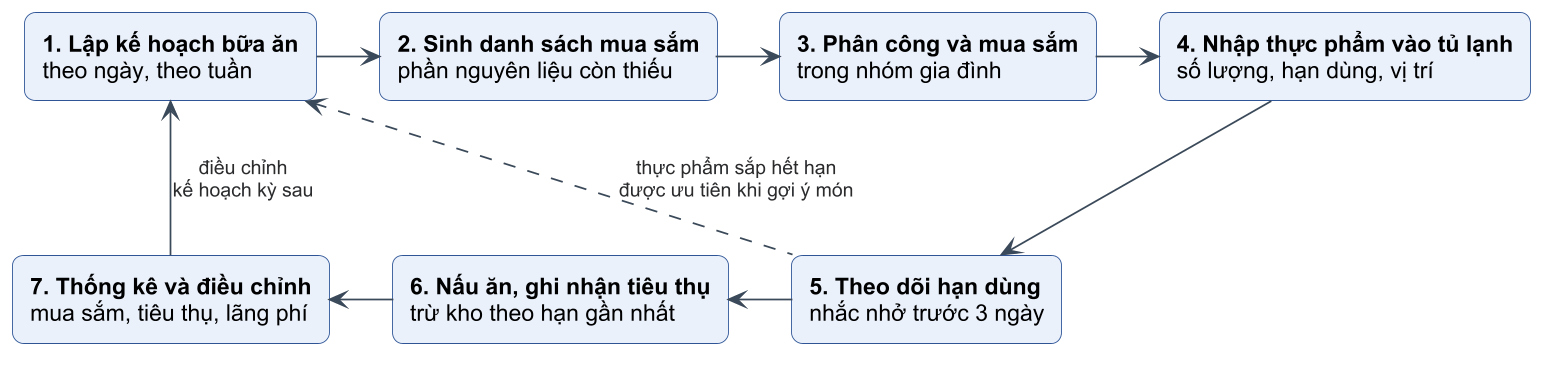
\includegraphics[width=\textwidth]{c1-02-chu-trinh-nghiep-vu.png}
\par\vspace{0.25cm}
\begin{columns}[T,onlytextwidth]
\column{0.49\textwidth}\key{Trong phạm vi}\\Cá nhân và nhóm gia đình.\\Mua sắm, bảo quản, lập bữa ăn, thống kê.
\column{0.47\textwidth}\key{Ngoài phạm vi}\\Đặt hàng, thanh toán và giao hàng.\\Tích hợp thiết bị tủ lạnh thông minh.
\end{columns}
\par\vspace{0.12cm}
\source{Chương 1, Hình chu trình nghiệp vụ và bảng phạm vi đề tài.}
\end{frame}
% 04 - 40 giây. Sơ đồ phân rã rút gọn, giữ đủ tám phân hệ.
\begin{frame}{Sơ đồ phân rã chức năng}
\centering
\begin{tikzpicture}[x=1cm,y=1cm]
\node[box,fill=hustprimary,text=white,text width=4.2cm,font=\bfseries] (root) at (7,0) {Ứng dụng “Đi chợ tiện lợi”};
\foreach \y/\num/\name/\desc in {1.25/1/{Tài khoản và nhóm gia đình}/{Xác thực, hồ sơ, phân vai},2.45/2/{Danh sách mua sắm}/{Lập danh sách, phân công, nhập tủ},3.65/3/{Thực phẩm trong tủ lạnh}/{Tồn kho, hạn dùng, tiêu thụ},4.85/4/{Công thức nấu ăn}/{Lưu món, đối chiếu nguyên liệu}} {
\node[box,text width=5.4cm] (l\num) at (3,-\y) {\textbf{\num. \name}\\{\footnotesize\desc}};
\draw[hustprimary,thick] (root.south) -- (7,-0.58) -- (6.2,-0.58) |- (l\num.east);
}
\foreach \y/\num/\name/\desc in {1.25/5/{Kế hoạch bữa ăn}/{Lên lịch, gợi ý món, xác nhận nấu},2.45/6/{Tìm kiếm và phân loại}/{Tìm thực phẩm, món ăn, lọc},3.65/7/{Thống kê báo cáo}/{Mua sắm, tiêu thụ, lãng phí},4.85/8/{Quản trị hệ thống}/{Tài khoản, danh mục, cấu hình}} {
\node[box,text width=5.4cm] (r\num) at (11,-\y) {\textbf{\num. \name}\\{\footnotesize\desc}};
\draw[hustprimary,thick] (root.south) -- (7,-0.58) -- (7.8,-0.58) |- (r\num.west);
}
\end{tikzpicture}
\source{Rút gọn từ sơ đồ phân rã chức năng ở Chương 1.}
\end{frame}
\section{Chương 2. Đặc tả yêu cầu}
% 05 - 45 giây
\begin{frame}{Chương 2. Tác nhân và quyền sử dụng}
\begin{columns}[T,onlytextwidth]
\column{0.57\textwidth}
\key{5 tác nhân chính}
\begin{tikzpicture}[x=1cm,y=1cm]
\node[box,text width=2.2cm] (u) at (4,0) {Người dùng};
\node[box,text width=2.2cm] (m) at (4,-1.35) {Thành viên nhóm};
\node[box,text width=2.2cm] (l) at (4,-2.7) {Trưởng nhóm};
\node[box,text width=2.2cm] (a) at (0.6,-1.35) {Quản trị viên};
\node[box,text width=2.2cm] (g) at (0.6,0) {Khách};
\draw[-{Triangle[open,length=3mm]},thick] (m)--(u);
\draw[-{Triangle[open,length=3mm]},thick] (l)--(m);
\draw[-{Triangle[open,length=3mm]},thick] (a.north east)--(u.south west);
\node[align=left,font=\footnotesize,text width=7.4cm,anchor=north west] at (-0.6,-3.3) {Mũi tên tam giác: kế thừa quyền.\\Khách là vai trò trước khi đăng nhập.};
\end{tikzpicture}
\column{0.40\textwidth}
\key{4 tác nhân phụ}
\begin{itemize}\setlength\itemsep{5pt}
\item Bộ lập lịch
\item Dịch vụ thông báo đẩy
\item Dịch vụ thư điện tử
\item CSDL sản phẩm mở
\end{itemize}
\par\vspace{0.12cm}
\key{Ranh giới dữ liệu}\\{\small Dữ liệu theo không gian cá nhân hoặc nhóm. Quản trị viên không xem nội dung riêng của gia đình.}
\end{columns}
\source{Chương 2, mục 2.1.1--2.1.2; quy tắc BR23.}
\end{frame}
% 06 - 45 giây
\begin{frame}{Bảng use case theo 9 nhóm chức năng}
\small
\renewcommand{\arraystretch}{1.13}
\begin{tabular}{@{}P{3.9cm}P{2.05cm}cP{6.45cm}@{}}\toprule
\textbf{Nhóm chức năng} & \textbf{Mã use case} & \textbf{Số} & \textbf{Chức năng đại diện}\\\midrule
1. Tài khoản & UC01--UC08 & 8 & Đăng ký, OTP, đăng nhập, thiết lập nhắc\\
2. Nhóm gia đình & UC09--UC15 & 7 & Tạo nhóm, mời, tham gia, chuyển quyền\\
3. Danh sách mua sắm & UC16--UC23 & 8 & Phân công, đánh dấu đã mua, nhập tủ\\
4. Tủ lạnh & UC24--UC31 & 8 & Thêm lô, ghi nhận dùng, nhắc hạn\\
5. Công thức nấu ăn & UC32--UC36 & 5 & Lưu công thức, đối chiếu nguyên liệu\\
6. Kế hoạch bữa ăn & UC37--UC41 & 5 & Lên lịch, gợi ý món, xác nhận đã nấu\\
7. Tìm kiếm và phân loại & UC42--UC43 & 2 & Tìm thực phẩm, món ăn, lọc danh mục\\
8. Thống kê báo cáo & UC44--UC47 & 4 & Chi tiêu, tiêu thụ, lãng phí, xuất tệp\\
9. Quản trị hệ thống & UC48--UC53 & 6 & Tài khoản, danh mục, tham số\\\bottomrule
\end{tabular}
\par\vspace{0.16cm}
\key{Tổng: 53 use case.} Tài khoản và nhóm gia đình tách thành 2 gói ở chương 2.
\source{Chương 2, bảng danh mục use case theo gói chức năng.}
\end{frame}
% 07 - 45 giây. Phân rã gói mua sắm, đủ UC16--UC23.
\begin{frame}{Biểu đồ use case: nhóm mua sắm}
\centering
\begin{tikzpicture}[x=0.96cm,y=0.86cm]
\draw[rounded corners,draw=hustprimary] (1.85,-6.55) rectangle (12.4,0.4);
\node[font=\small\bfseries,fill=white] at (7.2,0.4) {Quản lý danh sách mua sắm};
\node[uc,text width=2.7cm] (u16) at (4.2,-0.5) {UC16\\Tạo danh sách};
\node[uc,text width=2.7cm] (u23) at (4.2,-1.7) {UC23\\Xem lịch sử};
\node[uc,text width=2.7cm] (u17) at (4.2,-2.9) {UC17\\Sửa mặt hàng};
\node[uc,text width=3.0cm] (u20) at (4.2,-4.1) {UC20\\Đánh dấu đã mua};
\node[uc,text width=3.1cm] (u18) at (10,-0.9) {UC18\\Sao chép danh sách};
\node[uc,text width=3.1cm] (u22) at (10,-2.2) {UC22\\Sinh DS từ kế hoạch};
\node[uc,text width=3.1cm] (u21) at (10,-4.1) {UC21\\Chuyển vào tủ lạnh};
\node[uc,text width=2.8cm] (u19) at (10,-5.8) {UC19\\Phân công mua};
\node[font=\small\bfseries,align=center] (user) at (0.7,-2.2) {Người\\dùng};
\node[font=\small\bfseries,align=center] (leader) at (0.7,-5.8) {Trưởng\\nhóm};
\node[font=\footnotesize,align=center] (push) at (13.7,-5.8) {Dịch vụ\\thông báo đẩy};
\foreach \n in {u16,u23,u17,u20} \draw[black!65] (user.east)--(\n.west);
\draw[black!65] (user.south) -- (0.7,-5.2) -- (7,-5.2) -- (7,-2.2) -- (u22.west);
\draw[rel] (u18.west)--node[labeltext,above]{\guillemotleft extend\guillemotright}(u16.east);
\draw[rel] (u18.south west)--node[labeltext,below]{\guillemotleft extend\guillemotright}(u23.east);
\draw[rel] (u21.west)--node[labeltext,above]{\guillemotleft extend\guillemotright}(u20.east);
\draw[black!65] (leader)--(u19);\draw[black!65] (u19)--(push);
\end{tikzpicture}
\end{frame}
% 08 - 65 giây
\begin{frame}{UC20 và UC21: mua hàng và nhập tủ lạnh}
\key{Tác nhân:} Người dùng trong không gian hiện hành.
\smallnote{Điều kiện: danh sách chưa hoàn tất, mặt hàng cần mua hoặc đã phân công.}
\par\vspace{0.1cm}
\centering
\begin{tikzpicture}[node distance=0.5cm]
\node[box,text width=2.5cm] (a) {Chọn hàng\\\textbf{Đã mua}};
\node[box,text width=2.8cm,right=of a] (b) {Ghi người mua,\\số lượng thực tế};
\node[box,text width=2.55cm,right=of b] (c) {Nhập tủ\\Rà soát hạn};
\node[box,text width=2.6cm,right=of c] (d) {Tạo lô\\\textbf{Đã nhập tủ}};
\draw[flow](a)--(b);\draw[flow](b)--(c);\draw[flow](c)--(d);
\end{tikzpicture}
\par\par\vspace{0.35cm}\raggedright
\begin{columns}[T,onlytextwidth]
\column{0.49\textwidth}\key{Nhánh cần xử lý}
\begin{itemize}\item Hàng giao cho người khác: hỏi xác nhận mua hộ.\item Nhập tủ là lựa chọn mở rộng của UC20.\end{itemize}
\column{0.47\textwidth}\key{Kết quả và ràng buộc}
\begin{itemize}\item Mỗi mặt hàng sinh đúng một lô.\item Gửi lại yêu cầu không tạo lô trùng.\end{itemize}
\end{columns}
\par\vspace{0.2cm}
\source{Chương 2, đặc tả UC20--UC21. Luồng chính rút gọn.}
\end{frame}
% 09 - 70 giây
\begin{frame}{UC22: sinh danh sách từ kế hoạch bữa ăn}
\key{Luồng chính:} Chọn ngày, gộp nhu cầu, phân bổ tồn kho, xác nhận phần thiếu.
\smallnote{Điều kiện: có món chưa nấu gắn công thức. Chỉ tính lượng còn hạn đến ngày nấu và hàng chờ mua đến kịp.}
\par\vspace{0.12cm}
\begin{columns}[T,onlytextwidth]
\column{0.48\textwidth}
\key{Ví dụ trong báo cáo: cà rốt}
\renewcommand{\arraystretch}{1.4}
{\small\begin{tabular}{@{}P{2.7cm}P{3.9cm}@{}}\toprule
\textbf{Nhu cầu} & 0,4 kg ngày D; 0,6 kg ngày D+2\\\midrule
Lô A & 0,5 kg; hết hạn D+1\\
Lô B & 0,2 kg; hết hạn D+3\\
Đang chờ mua & 0,1 kg; mua trước D\\\bottomrule
\end{tabular}}
\column{0.48\textwidth}
\key{Phân bổ theo từng ngày}
\begin{itemize}\setlength\itemsep{6pt}
\item Ngày D: lấy 0,4 kg từ lô A.
\item Ngày D+2: phần còn lại của A đã quá hạn.
\item Lô B và hàng chờ mua đáp ứng 0,3 kg.
\end{itemize}
{\Large\color{hustprimary}\bfseries Cần mua thêm 0,3 kg}
\end{columns}
\par\vspace{0.15cm}
\smallnote{FEFO: ưu tiên lô hết hạn sớm. Mỗi lượng chỉ phân bổ một lần. Không thiếu thì không tạo danh sách.}
\source{Chương 2, UC22 và ví dụ kiểm chứng phần thiếu.}
\end{frame}
% 10 - 40 giây
\begin{frame}{UC31: tự động nhắc thực phẩm sắp hết hạn}
\key{Kích hoạt:} Bộ lập lịch chạy hằng ngày, mặc định 08:00.
\par\vspace{0.25cm}
\centering
\begin{tikzpicture}[node distance=0.55cm]
\node[box,text width=2.5cm] (a) {Kiểm tra hạn\\các lô còn lượng};
\node[box,text width=2.5cm,right=of a] (b) {Lọc theo\\từng thành viên};
\node[box,text width=2.5cm,right=of b] (c) {Lưu thông báo\\vào hộp thư};
\node[box,text width=2.5cm,right=of c] (d) {Gửi thông báo\\đến thiết bị};
\draw[flow](a)--(b);\draw[flow](b)--(c);\draw[flow](c)--(d);
\end{tikzpicture}
\par\par\vspace{0.4cm}\raggedright
\begin{columns}[T,onlytextwidth]
\column{0.47\textwidth}\key{Ngưỡng nhắc}\par Mặc định trước \textbf{3 ngày}.\\Cá nhân chọn từ 1 đến 7 ngày.
\column{0.49\textwidth}\key{Ngoại lệ}\par Tắt nhắc hoặc không có lô: bỏ qua.\\Lỗi gửi: thử lại tối đa 3 lần.
\end{columns}
\par\vspace{0.28cm}
\smallnote{Kết quả: mỗi thành viên nhận tối đa một thông báo tổng hợp mỗi ngày, không gửi trùng.}
\source{Chương 2, đặc tả UC31; BR12--BR13.}
\end{frame}
% 11 - 60 giây
\begin{frame}{UC40: gợi ý món từ thực phẩm sẵn có}
\key{Tác nhân:} Người dùng. \quad\key{Đầu ra:} Tối đa 10 món, kèm nguyên liệu còn thiếu.
\par\vspace{0.12cm}
\begin{columns}[T,onlytextwidth]
\column{0.43\textwidth}
\key{Cách xếp hạng}
\[S=0{,}6R+0{,}3E+0{,}1F\]
{\small
\textbf{R}: tỷ lệ nguyên liệu được đáp ứng.\par
\textbf{E}: ưu tiên thực phẩm sắp hết hạn.\par
\textbf{F}: món được đánh dấu yêu thích.}
\par\vspace{0.2cm}
\smallnote{Loại món dưới ngưỡng đáp ứng đã cấu hình. Tủ trống: hiển thị công thức mẫu.}
\column{0.53\textwidth}
\key{Ví dụ xếp hạng trong báo cáo}
\renewcommand{\arraystretch}{1.5}
{\small\begin{tabular}{@{}P{3.5cm}ccc@{}}\toprule
\textbf{Món ăn} & \textbf{R} & \textbf{E} & \textbf{S}\\\midrule
Canh chua cá lóc & 0,75 & 1 & \textbf{0,75}\\
Trứng xào cà chua & 1 & 0 & 0,60\\\bottomrule
\end{tabular}}
\smallnote{Giả sử cả hai món chưa được yêu thích, F = 0.}
\par\vspace{0.12cm}
Canh chua ưu tiên dùng cá lóc và dứa gần hết hạn, nhưng cần mua thêm me.
\end{columns}
\par\vspace{0.18cm}
\key{Gợi ý chỉ đọc dữ liệu.} UC41 trừ kho khi người dùng xác nhận đã nấu.
\source{Chương 2, đặc tả UC40 và ví dụ tính điểm gợi ý.}
\end{frame}
% 12 - 35 giây
\begin{frame}{Yêu cầu chất lượng và tiêu chí kiểm chứng}
\renewcommand{\arraystretch}{1.6}
\begin{tabular}{@{}P{3.15cm}P{10.6cm}@{}}\toprule
\textbf{Nhóm yêu cầu} & \textbf{Mục tiêu nghiệm thu}\\\midrule
Hiệu năng & Gợi ý món trong 2 giây; đồng bộ nhóm trong 3 giây\\
Độ tin cậy & Thao tác cốt lõi dùng được khi mất mạng; đồng bộ lại\\
Nhất quán dữ liệu & UC21 không nhập trùng; UC41 không trừ kho hai lần\\
Phân quyền & Máy chủ kiểm tra vai trò và không gian ở mọi API\\
Đa nền tảng & Một mã nguồn Flutter; Android 8.0+, iOS 13+\\\bottomrule
\end{tabular}
\par\vspace{0.3cm}
\key{Đây là yêu cầu cần kiểm thử, chưa phải kết quả đo thực tế.}
\source{Chương 2, NFR09--NFR11, NFR16, NFR19; UC21 và UC41.}
\end{frame}
% 13 - 10 giây. Nội dung: 560 giây; dự phòng chuyển người nói: 40 giây.
\begin{frame}{Tổng kết chương 1 và chương 2}
\par\vspace{0.45cm}
{\Large\key{Chương 1}}\par
Xác định bài toán, phạm vi và 8 phân hệ nghiệp vụ.
\par\vspace{0.35cm}
{\Large\key{Chương 2}}\par
Đặc tả 53 use case trong 9 nhóm và yêu cầu chất lượng.
\par\vspace{0.4cm}
\key{Trọng tâm:} Dữ liệu liên thông giữa mua sắm, tủ lạnh và bữa ăn.
\par\vspace{0.55cm}
{\Large\color{hustprimary}\bfseries Cảm ơn thầy và các bạn!}
\end{frame}
\end{document}
